\documentclass[11pt]{article}

% general
\usepackage{hyperref}
\hypersetup{colorlinks=true, citecolor=blue, linkcolor=blue, urlcolor=blue} % you can change colors here
\usepackage{natbib}

% tables and figures
\usepackage{booktabs}
\usepackage{float}

\usepackage{graphicx}
\usepackage[skip=10pt]{caption}
\usepackage{lscape}


\title{Title of your paper}
\author{Your name \\ Your university\thanks{\href{mailto:exmaple@example.com}{exmaple@example.com}.}} 
\date{August, 2018}



\begin{document}


\maketitle
\tableofcontents % add contents


\section{Examples}


\subsection{Itemization}

\begin{itemize}
\item Item 1
\item[] Item 2 % add [] to remove dots
	\begin{itemize}
	\item[i.] Item 2 (a)
	\item[ii.] Item 2 (b)
	\end{itemize}
\end{itemize}

\subsection{Text}

You can add an \underline{underline}. Add a footnote.\footnote{This is a footnote.} 

Cite a paper by writing a key \cite{ref1}, \citep{ref2} (See \href{http://merkel.texture.rocks/Latex/natbib.php}{this site}).

Use two slashes \\
to start a new line without an indent. 

If you want to add an indent before the new line, 

make a space above the line. \\
% lines with a percent mark are ignored
Change the font size:

\begin{itemize}
	\item {\footnotesize footnotesize}
	\item {\small small}
	\item {\large large}
	\item {\Large Large}
	\item {\LARGE LARGE}
	\item {\huge huge}
	\item {\Huge Huge}
\end{itemize}
Change the font style:

\begin{itemize}
	\item {\it Italic}
	\item {\bf Bold}
	\item {\rm Roman}
	\item {\sf Sans Serif}
	\item {\tt Typewriter}
	\item {\sc Small Caps}
	\item {\sl Slanted}
\end{itemize}

\subsection{Math}

Write a math expression like this $y = f(x)$, or:
\begin{equation}
	y = \alpha + \beta x + \epsilon. \label{eq:reg} % you can use greek letters
\end{equation}
If you want multile lines:
\begin{eqnarray}
	y &=& (x+1)^2 \label{eq:reg1} \nonumber \\ % \nonumber removes the equation number
  	 &=& x^2 + 2x + 1. \label{eq:reg2} 
\end{eqnarray}

You can refer to each equation in the text as you like (\autoref{eq:reg}, equation (\ref{eq:reg}), (\ref{eq:reg1}), (\ref{eq:reg2})).

Write special math symbols: $\leq, \geq, \neq, \rightarrow, \uparrow, \cap, \cup$, etc.

Write fractions:
\begin{equation}
	y = \frac{1 - x}{1 + x}.
\end{equation}

\subsection{Tables}

\begin{table}[H] %location h = here, t = top, b = bottom, p = a special page, H = precise location
	\caption{Summary statistics}
	\begin{center}
	\scalebox{0.9}[0.9]{
		\begin{tabular}{llllll}
\toprule
{} &      mean &       std &      min &   max & count \\
\midrule
uid           &   1281.48 &   736.896 &        1 &  2538 &  3392 \\
ELECYEAR      &   2011.56 &   1.98969 &     2009 &  2014 &  3392 \\
PREFEC        &   20.8821 &   12.2485 &        1 &    47 &  3392 \\
DISTRICT      &   5.77712 &   5.13715 &        1 &    25 &  3392 \\
PRBLOCK       &   58.8544 &   5.09346 &       51 &    66 &  2906 \\
INCUMB        &   1.79658 &  0.938328 &        1 &     3 &  3392 \\
TERM          &   1.45136 &   2.39026 &        0 &    16 &  3392 \\
SEX           &   1.15271 &  0.359763 &        1 &     2 &  3392 \\
AGE           &   50.5746 &   11.2587 &       25 &    94 &  3390 \\
RESULT        &    2.0339 &    1.2166 &        1 &     4 &  3392 \\
\bottomrule
\end{tabular}

	}
	\end{center}
	{\footnotesize {\it Notes}: Brabrabra.} \label{tab:sum_stat1}
\end{table}


\begin{table}[H] % add position if you like
\caption{OLS regressions}
\begin{center}
\begin{tabular}{lcc}
\hline
               & Model 1 & Model 2  \\
\midrule
\midrule
AGE            & 0.01*** & 0.01***  \\
               & (0.00)  & (0.00)   \\
PREFEC         &         & -0.00    \\
               &         & (0.00)   \\
Intercept      & 2.47*** & 2.48***  \\
               & (0.13)  & (0.14)   \\
R-squared      & 0.008   & 0.008    \\
Number of obs. & 2157    & 2157     \\
\hline
\end{tabular}
\end{center}
{\footnotesize {\it Notes}: Standard errors in parentheses. $^{*} p < 0.1, ^{**} < 0.05, ^{***} < 0.01$.} \label{tab:ols1}
\end{table} 

You can refer to each table in the text as you like (\autoref{tab:ols1}, table \ref{tab:ols1}, \ref{tab:sum_stat1}).

\subsection{Figures}


\begin{figure}[H] 
	\begin{center}
	\caption{Political candidates' opinion about fiscal policy} 
	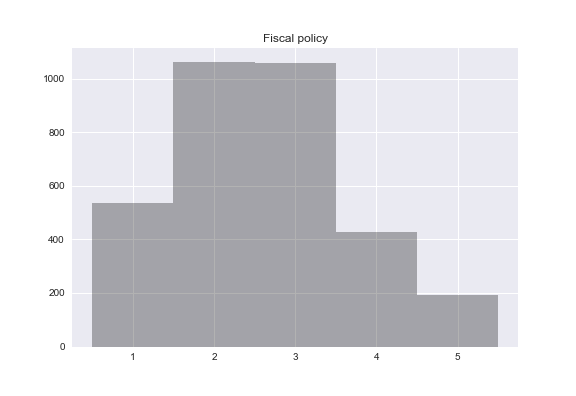
\includegraphics[width=0.7\textwidth]{yn_fiscalpol_py.png} \label{fig:hist1}
	\end{center}	
	 \vspace{-5mm}
	{\footnotesize {\it Notes}: Brabrabra.}
\end{figure}

%\begin{landscape} % make a figure vertical

\begin{figure}[H]
	\begin{center}
	\caption{Political candidates' opinion about fiscal policy, by sex} 
	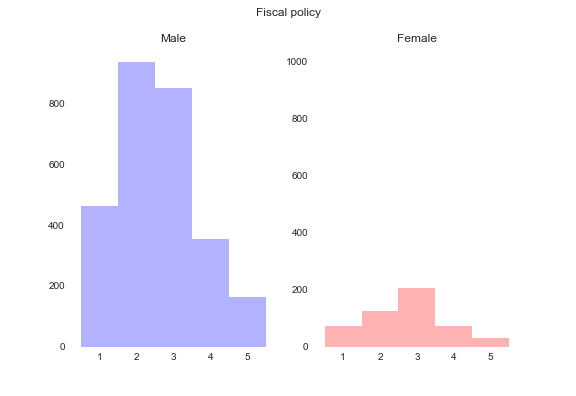
\includegraphics[width=0.7\textwidth]{yn_fiscalpol_bysex_py.png} \label{fig:hist2} 
	\end{center}
	\vspace{-5mm}
	{\footnotesize {\it Notes}: Brabrabra.}
\end{figure}

%\end{landscape}

You can refer to each figure in the text as you like (\autoref{fig:hist1}, figure (\ref{fig:hist1}), (\ref{fig:hist2})).

\bibliographystyle{chicago} % compile whenever you update the bibtex file using BibTeX above, then compile again using pdfLaTeX
\bibliography{ref_list}

\end{document}